\subsection{1.1 Unit conversions}
	\begin{itemize}
		\itemsep0em
		\raggedright
  		\item \textbf{Energy:} $1eV=1.602\cdot 10^{-19}J$,    $1cal=4.18J$
    	\item \textbf{Pressure:} $P = \frac{F}{A} = \rho \cdot h \cdot g$\\ $1 \textrm{atm} = 760mm \; \textrm{Hg} = 760 \textrm{torr} = 101'325 \textrm{Pa} = 1.01325 \textrm{bar}$\\ Manometer: $P = P_{atm}\pm \rho g h$
    	\item \textbf{Force:} $F = m \cdot g, \; m = \rho \cdot V$
		\item \textbf{Amount of substance:} $1 \textrm{mol} = 6.022\cdot 10^{23} \textrm{(Avogadro)}$
    	\item \textbf{Length:} $1\text{Å}=10^{-10}m$
    	\item \textbf{STP; } $0\tccentigrade = 273.15K, \; 1atm; \; V_m = 22.41L$
	\end{itemize}

\subsection{1.2 General}
    \begin{itemize}
		\itemsep0em
        \item \textbf{Kinetic energy:} $E_{kin} = \frac{1}{2} \cdot m \cdot v^2$
        \item \textbf{Potential energy:} $E_{pot} = m \cdot g \cdot \Delta h$
        \item \textbf{electrostatic:} $E_{el}=\frac{\kappa Q_1Q_2}{d^2}$\quad $\kappa = \frac{1}{4\pi \epsilon_0}$
        \item \textbf{Photon energy: } $E_\gamma = h\cdot f = \frac{h\cdot c}{\lambda}$
        \item \textbf{De Broglie wavelength: } $\lambda = \frac{h}{m\cdot v}$
    \end{itemize}
    	
\subsection{1.3 Trends in the periodic table of elements}
	\begin{itemize}
		\itemsep0em
    	\item \textbf{Ionisation energy: }The ionization energy is the quantity of energy that an isolated, gaseous atom in the ground electronic state must absorb to discharge an electron, resulting in a cation.
    	\item \textbf{Electron affinity: }Electron affinity is defined as the change in energy (in kJ/mole) of a neutral atom (in the gaseous phase) when an electron is added to the atom to form a negative ion.
    	\item \textbf{Electronnegativity:} Electronegativity is a measure of an atom's ability to attract shared electrons to itself.
	\end{itemize}
	\centerline{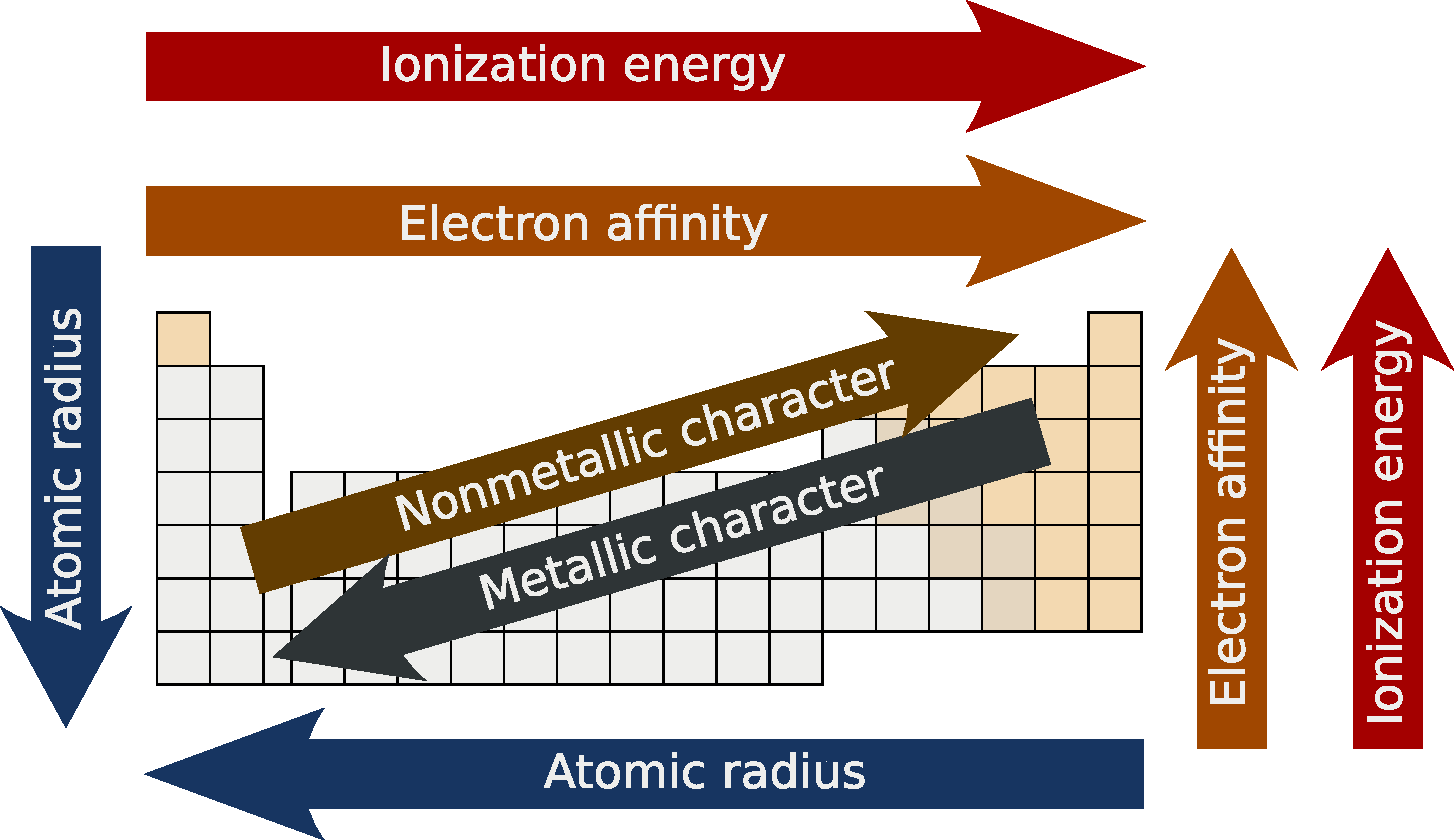
\includegraphics[width=0.65\linewidth]{src/1_Basics/Periodic_trends.pdf}}
	\vspace*{0.5em}